\documentclass{beamer}

\setbeamertemplate{caption}{\raggedright\insertcaption\par}

\mode<presentation>
{
  \usetheme{CambridgeUS}

  \setbeamercovered{transparent}
}


\definecolor{Or}{RGB}{255,153,000}
\definecolor{Indigo}{RGB}{72,61,139}
\definecolor{Magenta}{RGB}{139,0,139}

\setbeamercolor{normal text}{fg=black,bg=white}
\setbeamercolor{alerted text}{fg=Indigo}
\setbeamercolor{example text}{fg=Indigo}

%\setbeamercolor{background canvas}{fg=myforeground, bg=white}
%\setbeamercolor{background}{fg=myforeground, bg=mybackground}
%
%\setbeamercolor{palette primary}{fg=black, bg=gray!30!white}
%\setbeamercolor{palette secondary}{fg=black, bg=gray!20!white}
%\setbeamercolor{palette tertiary}{fg=black, bg=gold}



\setbeamercolor{palette tertiary}{fg=black, bg=Indigo}
\setbeamercolor{frametitle}{fg=Indigo}
\setbeamercolor{title}{fg=Indigo}
\setbeamercolor{footline}{fg=Indigo, bg=Indigo}
\setbeamercolor{author in head/foot}{fg=black}
\setbeamercolor{date in head/foot}{fg=black}
\setbeamercolor{title in head/foot}{fg=black}

\definecolor{Highlight}{RGB}{139,0,139}
\newcommand{\HL}[1]{{\color{Highlight}#1}}

\usefonttheme{professionalfonts}
\beamertemplatenavigationsymbolsempty

\usepackage[english]{babel}
\usepackage{color}
\usepackage{amsfonts}
\usepackage{amssymb}
\usepackage{epsfig}
\usepackage{amsmath}
\usepackage{txfonts}
\usepackage{relsize}

\usepackage{natbib}
\usepackage{bibentry}
\bibliographystyle{apalike}
\usepackage{tikz}
\usetikzlibrary{decorations.pathreplacing}

\newcommand\footcite[1]{\footnote{\bibentry{#1}}\label{\thepage:#1}}
\newcommand\secondcite[1]{\textsuperscript{\ref{\thepage:#1}}}

%\usepackage{bbold}
\usepackage{dsfont}
\usepackage{bbm}

\usepackage[latin1]{inputenc}

\newcommand{\id}{\mathbbm{1}}
\newcommand{\HH}{\mathcal{H}}
\newcommand{\CC}{\mathbb{C}}
\newcommand{\BB}{\mathcal{B}}
\newcommand{\dd}{\mathrm{d}}
\newcommand{\UU}{\mathcal{U}}
\newcommand{\ZZ}{\mathbb{Z}}
\newcommand{\tr}{\mathrm{tr}}
\newcommand{\Tr}{\mathrm{Tr}}
\renewcommand{\AA}{\mathcal{A}}

\newcommand{\mean}[1]{\langle #1 \rangle}
\newcommand{\cumul}[1]{\langle\!\langle #1 \rangle\!\rangle}

\DeclareRobustCommand{\augiefamily}{%
  \fontfamily{augie}\fontseries{m}\fontshape{n}\selectfont}
\DeclareTextFontCommand{\textaugie}{\augiefamily}

\usepackage{physics}

\setlength{\parskip}{0.1cm}

\title[SPT classification]%\hspace{1cm} \insertframenumber/\inserttotalframenumber]
{SPT classification:\\from the AKLT model to recent proofs}

\author[Tijl]
{Tijl Jappens \\
 \scriptsize KU Leuven}


\institute[]{
instituut voor theorethische fysica KU Leuven
}


\date{\today}

\setbeamertemplate{itemize items}{\color{black}$\triangleright$}
\setbeamertemplate{enumerate items}{\color{black}\insertenumlabel.}

\usepackage[T1]{fontenc}
\DeclareRobustCommand{\augiefamily}{%
  \fontfamily{augie}\fontseries{m}\fontshape{n}\selectfont}
\DeclareTextFontCommand{\textaugie}{\augiefamily}

\begin{document}
\nobibliography{SPT_Presentation}

%%%%%%%%%% Removes the frame number from the title page %%%%%%%%%%
\bgroup
\makeatletter
\setbeamertemplate{footline}
{
  \leavevmode%
  \hbox{%
  \begin{beamercolorbox}[wd=.333333\paperwidth,ht=2.25ex,dp=1ex,center]{author in head/foot}%
 %   \usebeamerfont{author in head/foot}\insertshortauthor\expandafter\beamer@ifempty\expandafter{\beamer@shortinstitute}{}{~~(\insertshortinstitute)}
  \end{beamercolorbox}%
  \begin{beamercolorbox}[wd=.333333\paperwidth,ht=2.25ex,dp=1ex,center]{title in head/foot}%
%    \usebeamerfont{title in head/foot}\insertshorttitle
  \end{beamercolorbox}%
  \begin{beamercolorbox}[wd=.333333\paperwidth,ht=2.25ex,dp=1ex,right]{date in head/foot}%
%    \usebeamerfont{date in head/foot}\insertshortdate{}\hspace*{2em}
%    \insertframenumber{} / \inserttotalframenumber\hspace*{2ex} 
  \end{beamercolorbox}}%
  \vskip0pt%
}
\makeatother
\begin{frame}
\titlepage
\end{frame}
\egroup

\setcounter{framenumber}{0}
\begin{frame}{The singlet and the triplet}
	\begin{block}{On site Hilbert space}
		In $\CC^4\cong \CC^2\times \CC^2$, take as basis
		\begin{align*}
			&&\ket{s}&=\frac{1}{\sqrt{2}}(\ket{\uparrow\downarrow}-\ket{\downarrow\uparrow})&&\\
			\ket{0}&=\frac{1}{\sqrt{2}}(\ket{\uparrow\downarrow}+\ket{\downarrow\uparrow})&\ket{-1}&=\ket{\downarrow\downarrow}&\ket{1}&=\ket{\uparrow\uparrow}.
		\end{align*}
	\end{block}
	\pause
	\begin{block}{Group action}
		Take $U\in \textrm{Hom}(\ZZ^2\times \ZZ^2,U(\CC^4))$ by setting
		\begin{align*}
		U(-1,1)&=\sigma_x\otimes \sigma_x&U(1,-1)&=-\sigma_y\otimes \sigma_y&U(-1,-1)&=\sigma_z\otimes \sigma_z.
		\end{align*}
	\end{block}
\end{frame}

\begin{frame}{The singlet and the triplet}
	\begin{block}{Group action}
		Take $U\in \textrm{Hom}(\ZZ^2\times \ZZ^2,U(\CC^4))$ by setting
		\begin{align*}
		U(-1,1)&=\sigma_x\otimes \sigma_x&U(1,-1)&=-\sigma_y\otimes \sigma_y&U(-1,-1)&=\sigma_z\otimes \sigma_z.
		\end{align*}
	\end{block}
	Think of $\ZZ^2\times \ZZ^2$ as a subgroup of $SO(3)$ where
	\begin{itemize}
		\item $(-1,1)$ rotates around $x$-axis by $\pi$ radial.
		\item $(1,-1)$ rotates around $y$-axis by $\pi$ radial.
		\item $(-1,-1)$ rotates around $z$-axis by $\pi$ radial.
	\end{itemize}
	\pause
	\begin{block}{Back to the state}
		$\ket{s}$ transforms one dimensional under $\ZZ^2\times \ZZ^2$.\\
		$\ket{-1},\ket{0},\ket{1}$ transform irreducibly under $\ZZ^2\times \ZZ^2$.
	\end{block}
\end{frame}

\begin{frame}{Intermezzo linear and projective representations}
	We had a (linear) representation
	\begin{align*}
			U(-1,1)&=\sigma_x\otimes \sigma_x&U(1,-1)&=-\sigma_y\otimes \sigma_y&U(-1,1)&=\sigma_z\otimes \sigma_z.
	\end{align*}
	\pause
	Does this reduce to a representation on $\CC^2$?\\
	\pause
	In particular, if one takes
	\begin{align}
		U(-1,1)&=\sigma_x&U(1,-1)&=\sigma_y&U(-1,-1)&=\sigma_z
	\end{align}
	then
	\begin{equation}
		U(-1,1)U(1,-1)=-U(1,-1)U(-1,1)=i U(-1,-1).
	\end{equation}
	It is a projective representation.
\end{frame}

\begin{frame}{The (fake) AKLT model}
	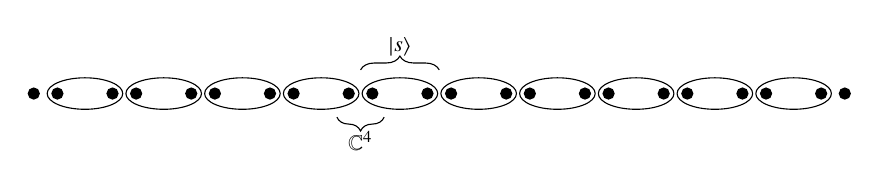
\begin{tikzpicture}
		\foreach \i in {1,...,10}
		{
			\draw[black] (\i+0.5,0) ellipse (0.48 and 0.2);
			\filldraw [black] (\i-0.15,0) circle (2pt);
			\filldraw [black] (\i+0.15,0) circle (2pt);
			
		}
		\filldraw [black] (11-0.15,0) circle (2pt);
		\filldraw [black] (11+0.15,0) circle (2pt);
		\draw [decorate,decoration={brace,amplitude=5pt},xshift=0cm,yshift=0pt] (5,0.3) -- (5+1,0.3) node [black,midway,yshift=0.3cm] {\footnotesize $\ket{s}$};
		\draw [decorate,decoration={brace,amplitude=5pt},xshift=0cm,yshift=0pt] (5+0.3,-0.3) -- (5-0.3,-0.3) node [black,midway,yshift=-0.3cm] {\footnotesize $\CC^4$};
	\end{tikzpicture}\\
	On $\bigotimes_{i=1}^L(\CC^4)$, define a state
	\begin{equation}
		\ket{\psi}=\bigotimes_{i=1}^L\ket{s}_{(i,R),(i+1,L)}
	\end{equation}
	\pause
	It satisfies that:
	\begin{itemize}
		\item If I count the sites differently, this is a product state but if I take the sites in this way, it is not.
		\item If I put this state on closed boundary conditions it is invariant under
		\begin{equation}
			U(g)=\bigotimes_i U_i(g).
		\end{equation}
	\end{itemize}
\end{frame}

\begin{frame}{The (fake) AKLT model}
	Let us forget the boundaries for a while and define\\$\:$\\
	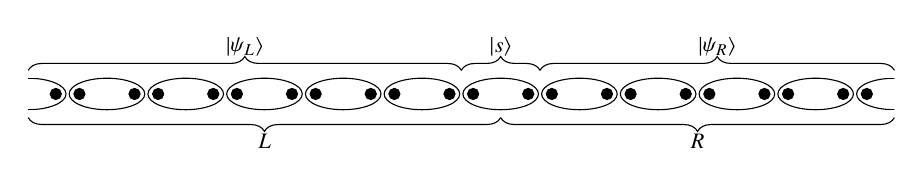
\begin{tikzpicture}
		\foreach \i in {1,...,10}
		{
			\draw[black] (\i+0.5,0) ellipse (0.48 and 0.2);
			\filldraw [black] (\i-0.15,0) circle (2pt);
			\filldraw [black] (\i+0.15,0) circle (2pt);
			
		}
		\filldraw [black] (11-0.15,0) circle (2pt);
		\filldraw [black] (11+0.15,0) circle (2pt);
		\begin{scope}
			\clip(0.5,0.2)rectangle(1,-0.2);
			\draw[black] (0.5,0) ellipse (0.48 and 0.2);
		\end{scope}
		\begin{scope}
			\clip(11,0.2)rectangle(11.5,-0.2);
			\draw[black] (11.5,0) ellipse (0.48 and 0.2);
		\end{scope}
		\draw [decorate,decoration={brace,amplitude=5pt},xshift=0cm,yshift=0pt] (7,0.3) -- (11.5,0.3) node [black,midway,yshift=0.3cm] {\footnotesize $\ket{\psi_R}$};
		\draw [decorate,decoration={brace,amplitude=5pt},xshift=0cm,yshift=0pt] (0.5,0.3) -- (6,0.3) node [black,midway,yshift=0.3cm] {\footnotesize $\ket{\psi_L}$};
		\draw [decorate,decoration={brace,amplitude=5pt},xshift=0cm,yshift=0pt] (6,0.3) -- (7,0.3) node [black,midway,yshift=0.3cm] {\footnotesize $\ket{s}$};
		\draw [decorate,decoration={brace,amplitude=5pt},xshift=0cm,yshift=0pt] (6.5,-0.3) -- (0.5,-0.3)  node [black,midway,yshift=-0.3cm] {\footnotesize $L$};
		\draw [decorate,decoration={brace,amplitude=5pt},xshift=0cm,yshift=0pt] (11.5,-0.3) -- (6.5,-0.3)  node [black,midway,yshift=-0.3cm] {\footnotesize $R$};
	\end{tikzpicture}
	\begin{block}{Claim}
		There does not exist any 
	\end{block}
\end{frame}

\begin{frame}{The AKLT model}
On $\HH:=\bigotimes_{n=1}^L\CC^3$ we define the AKLT Hamiltonian: 
\begin{equation*}
H_{\text{AKLT}}:= \sum_{i=1}^L\left(\vec{S}_i\cdot \vec{S}_{i+1}+\frac{1}{3}(\vec{S}_i\cdot \vec{S}_{i+1})^2\right).
\end{equation*}
\pause
This has some important properties:
\begin{itemize}
\item It has a unique gapped groundstate (construction wil follow).
\pause
\item It has an $SO(3)$ symmetry (we won't use this full symmetry).
\pause
\item It has in particular a $\ZZ_2\times \ZZ_2$ symmetry.
\end{itemize}
\end{frame}

\begin{frame}{The AKLT model}
On $\HH:=\bigotimes_{n=1}^L\CC^3$ we define the AKLT Hamiltonian: 
\begin{equation*}
H_{\text{AKLT}}:= \sum_{i=1}^L\left(\vec{S}_i\cdot \vec{S}_{i+1}+\frac{1}{3}(\vec{S}_i\cdot \vec{S}_{i+1})^2\right).
\end{equation*}
The action of this $\ZZ_2\times \ZZ_2$ symmetry is
\begin{align*}
U(1,0)&:=\exp(i\pi S^x)=\begin{pmatrix}0&0&-1\\0&-1&0\\-1&0&0\end{pmatrix}&U(0,1)&:=\exp(i\pi S^z)=\begin{pmatrix}-1&0&0\\0&1&0\\0&0&-1\end{pmatrix}
\end{align*}
on each site.
\end{frame}

\begin{frame}{The AKLT model}
On $\HH:=\bigotimes_{n=1}^L\CC^3$ we define the AKLT Hamiltonian: 
\begin{equation*}
H_{\text{AKLT}}:= \sum_{i=1}^L\left(\vec{S}_i\cdot \vec{S}_{i+1}+\frac{1}{3}(\vec{S}_i\cdot \vec{S}_{i+1})^2\right).
\end{equation*}
\begin{block}{Question:}
Is it possible to continuously deform the AKLT ground state to a product state while:
\begin{itemize}
\item keeping the gap open.
\item using only local operators.
\item preserving the symmetry.
\end{itemize}
\end{block}
\pause
It turns out the answer is no.
\end{frame}

\begin{frame}{AKLT groundstate is matrix product state}
It turns out we can write the AKLT groundstate as
\begin{equation*}
\ket{\psi}=\sum_{i_1,\cdots,i_L}\textrm{Tr}_{\CC^2}\left(A^{i_1}\cdots A^{i_L}\right)\ket{i_1,\cdots ,i_L}
\end{equation*}
where
\begin{align*}
A^+&:=\frac{1}{\sqrt{2}}\sigma^+&A^0&:=-\frac{1}{2}\sigma^z&A^-&:=-\frac{1}{\sqrt{2}}\sigma^-.
\end{align*}
\pause
This is invariant under the group action because
\begin{align*}
\sum_j (U(1,0) )_{ij}A^j&=\sigma^x A^i \sigma^x&\sum_j (U(0,1) )_{ij}A^j&=\sigma^z A^i \sigma^z.
\end{align*}
\end{frame}

\begin{frame}{Why is the AKLT ground state nontrivial?}
Some remarkts:
\begin{itemize}
\item $\sigma^x$ is a representation of $\ZZ^2$.
\pause
\item $\sigma^z$ is also a representation of $\ZZ^2$.
\pause
\item $\sigma^z\sigma^x=-\sigma^x\sigma^z=\sigma^y$.
\pause
\item Let $R(1,0)=\sigma^x$ and $R(0,1)=\sigma^z$. There does not exists a $\beta\in U(1)$ such for $R(1,1)=\beta \sigma^y$, R is a (linear representation).
\pause
\item For a product state $\bigotimes_{n=1}^L\ket{0}$, the $A's$ are
\[A^i=\delta_{i,0}\begin{pmatrix}1&0\\0&0\end{pmatrix}\]
and these transform as a linear representation (We took $\ket{0}$ because it is the simultanious eigenstate of $S^x$ and $S^z$.).
\end{itemize}
\end{frame}

\begin{frame}{Why is the AKLT ground state nontrivial?}
\begin{block}{Conclusion}
If there is an index, protecting phases invariant under $\ZZ_2\times\ZZ_2$ based on projective representations then the AKLT groundstate cannot be connected to a product state.
\end{block}
\end{frame}

\begin{frame}{Second group cohomology group}
Let $G$ be a compact group.
\begin{block}{Definition}
Take $R:G\rightarrow U(\CC^D)$. $R$ is the lift of a projective representation if there exists a $C:G^2\rightarrow U(1)$ satisfying
\[R(g)R(h)=C(g,h)R(gh).\]
\end{block}
\pause
Because of associativity
\begin{align*}
(R_n(g)R_n(h))R_n(l)&=R_n(g)(R_n(h)R_n(l))\\
C(g,h)C(gh,l)&=C(g,hl)C(h,l).
\end{align*}
Such a C is called a 2-cochain ($C\in Z^2$).
\end{frame}

\begin{frame}{Second group cohomology group}
\begin{block}{Definition}
We call $C:G^2\rightarrow U(1)$ a coboundary ($C\in B^2$) if there exists a $\beta:G\rightarrow U(1)$ such that
\[C(g,h)=\beta(g)\beta(h)\overline{\beta(gh)}.\]
\end{block}
The second group cohomology group is defined as $H^2(G,U(1)):=Z^2/B^2$.
\pause
\begin{block}{Claim}
The AKLT groundstate cannot be connected to a product state because cochain corresponding to
\begin{align*}
R(1,0)&=\sigma^x&R(0,1)&=\sigma^z&R(1,1)&=\sigma^y
\end{align*}
is in a nontrivial second group cohomology class.
\end{block}
\end{frame}

\begin{frame}{Matrix product state}
Translation invariance of AKLT state not important. We can make a more general, nonuniform construction:
\begin{columns}
\begin{column}{0.5\textwidth}
\[\HH := \bigotimes_{n=1}^{L}\CC^{d}.\]
\end{column}
\begin{column}{0.5\textwidth}
\begin{itemize}
\item $L$ is chain length.
\item $d$ is on site dimension.
\end{itemize}
\end{column}
\end{columns}
\pause
\begin{block}{Definition: Matrix product state (MPS)}
$\ket{\psi}\in\HH$ is a MPS (with periodic boundary) if $\exists D<<L:\forall n\in\{0,..,L\}:\forall i\in\{1,..,d\}:\exists A^i_n\in\BB(\CC^D):$
\begin{equation}
\ket{\psi}=\sum_{i_1,..,i_L}\Tr(A^{i_1}_1\cdots A^{i_L}_L)\ket{i_1,\cdots i_L}.
\end{equation}
\end{block}
\pause
\begin{itemize}
\item D is called bond dimension.
\end{itemize}
\end{frame}

\begin{frame}{On site group action}
For any $G$, a compact group we can take any representation:
\begin{align}
U(g)&\in\textrm{Hom}(G,U(\CC^d))&\tilde U(g)&:= \bigotimes_{n=0}^L U(g).
\end{align}
\pause
\begin{block}{Definition}
We say that an MPS $\ket{\psi}$ is $G$-invariant if $\exists \tilde{\alpha}\in\textrm{Hom}(G,U(1)):$
\[\tilde{U}(g)\ket{\psi}=\tilde{\alpha}(g)\ket{\psi}.\]
\end{block}
\end{frame}

\begin{frame}{On site group action on MPS}
\begin{block}{Lemma:}
Let $\ket{\psi}$ be an SPT then $\forall n\in\{1,L\}:$ $\exists R_n:G\rightarrow U(\CC^D)$ and $\alpha_n:G\rightarrow U(1)$ such that
\begin{equation}
\sum_{j=0}^{d}U(g)_{ij}A^j_n=\alpha_n(g) R_n(g)^\dagger A^i_n R_{n+1}(g)
\end{equation}
for all $g\in G.$
\end{block}
\pause
\begin{itemize}
\item $\alpha_n$ is a $U(1)$ representation.
\item $R_n$ is lift of projective representation.
\end{itemize}
\end{frame}

\begin{frame}{$C_n$ is uniform}
Since $U(gh)^\dagger U(g)U(h)=\id$ we need
\begin{equation}
A_n^i=R_n(h)^\dagger R_n(g)^\dagger R_{n}(gh) A^i_n R_{n+1}(gh)^\dagger R_{n+1}(g) R_{n+1}(h)
\end{equation}
and therefore $C_n(g,h)=C_{n+1}(g,h)$. From now on:
\[C_1(g,h)=\cdots=C_L(g,h)=C(g,h).\]
\pause
Therefore uniformity of (equivalences of) cochain comes about naturally.
\pause
\begin{block}{Claim}
Let $C$ be the cochain defined up to now then $(C)_\sim$ is independent of the choice of $R_n$ and $\alpha_n$.
\end{block}
\pause
One dimensional SPT's are classified by an $H^2(G,U(1))-$valued index.
\end{frame}

\begin{frame}{Translation invariance}
\begin{itemize}
\item The $\alpha_n(g)$ were not uniform.
\pause
\item What happens in the case where we impose translation invariance?
\end{itemize}
Eg. We set $d=2$ and $G=\ZZ_2$.\pause We let the on site group action be (for the $g\neq \text{id}$)
\[U(g)=\begin{pmatrix}1&0\\0&-1\end{pmatrix}.\]
\pause
\begin{block}{Claim:}
I cannot connect the states
\begin{align*}
\ket{\psi_\uparrow}&=\ket{\uparrow,\cdots,\uparrow}&\ket{\psi_\downarrow}&=\ket{\downarrow,\cdots,\downarrow}
\end{align*}
through local $G$ and translation invariant hamiltonians.
\end{block}
\end{frame}

\begin{frame}{Translation invariance}
A translation invariant MPS is of the form
\[\ket{\psi}=\sum_{i_1\cdots i_L}\textrm{Tr}(A^{i_1}\cdots A^{i_L})\ket{i_1,\cdots i_L}.\]
\pause
We still have $\exists \alpha\in\text{Hom}(G,U(1))$ and $R:G\rightarrow U(\CC^D)$ such that
 \[\sum_j U(g)_{ij}A^j=\alpha(g) R(g)^\dagger A^i R(g).\]
\pause
\begin{block}{Claim}
There exists an
\[H^2(G,U(1))\oplus \text{Hom}(G,U(1))=H^2(G,U(1))\oplus H^1(G,U(1))\]
valued index.
\end{block}
\end{frame}

\begin{frame}{Loops of SPT's}
Let
\begin{align}
H(\lambda)&= \sum_i H_i(\lambda)&U(\lambda)&= \mathcal{T}\exp(-i\int_0^\lambda \dd s H(s))
\end{align}
where each therm is $G-$invariant:
\[[H_i(\lambda),\tilde{U}(g)]=0.\]
\pause
Let $\ket{\psi}$ be a $G$-invariant MPS such that
\[U(1)\ket{\psi}\propto \ket{\psi}.\]
\end{frame}

\begin{frame}{Loops of SPT's: Making cuts}
\begin{columns}
\begin{column}{0.6\textwidth}
\onslide<1->{
\begin{align*}
H_R(\lambda)&=\sum_i H_i(\lambda)\chi(\textrm{supp}(H_i(\lambda))\subset R)\\
U_R(\lambda)&=\mathcal{T}\exp(-i \int_0^\lambda \dd s\: H_R(s) ).
\end{align*}
}
\onslide<2->{
Define
\[\ket{\psi_R}:= U_R(1)\ket{\psi}.\]
\begin{block}{Claim:}
\begin{itemize}
\item $\ket{\psi_R}$ is $G$-invariant and has same $\tilde{\alpha}(g)$.
\item $\ket{\psi_R}$ only differs from $\ket{\psi}$ around $B_1$ and $B_2$.
\end{itemize}
\end{block}
}
\end{column}
\onslide<1->{
\begin{column}{0.4\textwidth}
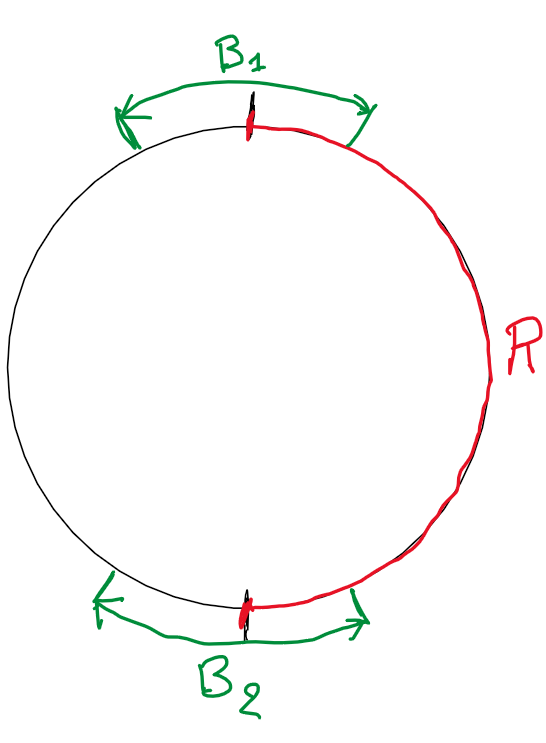
\includegraphics[width=\textwidth]{CircleRegions.png}
\end{column}
}
\end{columns}
\end{frame}

\begin{frame}{Loops of SPT's: Finite depth quantum cirquit}
A finite depth quantum cirquit (of depth 2) is of the form:
\begin{figure}
\center
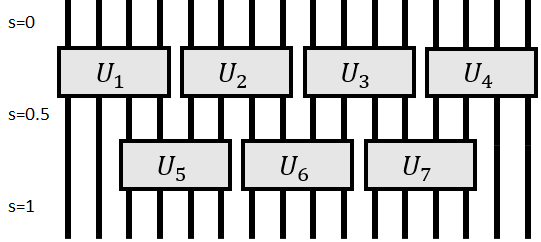
\includegraphics[width=0.8\textwidth]{FiniteDepthQuantumCirquit.png}
\end{figure}
\end{frame}

\begin{frame}{Loops of SPT's: Making previous statement precise}
\begin{columns}
\begin{column}{0.6\textwidth}
\begin{block}{Claim 1:}
Let $U_R(\lambda)$ be a finite depth quantum cirquit. $\exists\: B_1,B_2:\forall n\in B_1\cup B_2:\exists A'^i_n:$ such that $\ket{\psi_R}$ is $\ket{\psi}$ with the $A_n^i$ in $B_1\cup B_2$ replaced by $A'^i_n$.
\end{block}
\onslide<2->{
\begin{block}{Claim 2:}
Let $\ket{\psi_{1,R}}$ be the MPS that is $\ket{\psi}$ with the $A^i_n$ replaced by $A'^i_n$ in $B_1$ only then $\ket{\psi_{1,R}}$ is $G$-invariant as well.
\end{block}
}
\onslide<3->{
However $\tilde{\alpha}_1(g)/\tilde{\alpha}(g)$ need not be $1$. 
\[\tilde{\alpha}_1(g)/\tilde{\alpha}(g)\in H^1(G,U(1))\]
is called the charge pumping index.
}
\end{column}
\onslide<1->{
\begin{column}{0.4\textwidth}
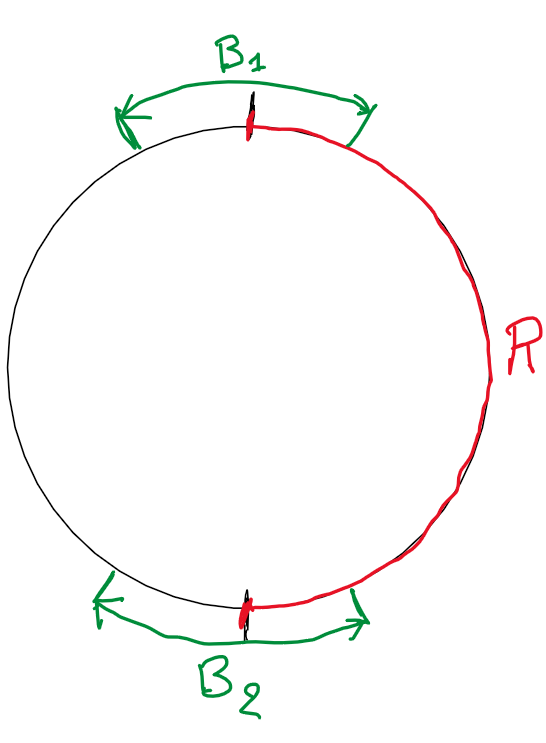
\includegraphics[width=\textwidth]{CircleRegions.png}
\end{column}
}
\end{columns}
\end{frame}

\begin{frame}{Quasi Local $C^*$ algebra}
Take
\begin{itemize}
\item $d$ the on site dimension.
\item $D$ the spatial dimension.
\item $\mathfrak{B}_{\ZZ^D}$ the local subsets of $\ZZ^D$.
\end{itemize}
\pause
We define the local $C^*$ algebra as follows: $\forall Z\in \mathfrak{B}_{\ZZ^D}\}:$
\begin{align*}
 \AA_Z&:=\bigotimes_{i\in Z}\left(\BB(\CC^d)\right)_i&\onslide<3->{\AA_{\text{loc}}&:=\{\AA_{Z} | Z\in \mathfrak{B}_{\ZZ^D}\}}.
\end{align*}
\onslide<4->{
\begin{block}{Definition: Quasi Local $C^*$ algebra}
We define $\AA$ as the norm closure of $\AA_{\text{loc}}$:
\[\AA:=\overline{\AA_{\text{loc}}}.\]
\end{block}}
\end{frame}

\begin{frame}{States and interactions}
$\omega:\AA\rightarrow \CC$ is a state if it is positive and linear.\\
\pause
\begin{itemize}
\item When will we say that two pure states are connected?
\pause
\item We won't define a topology only an equivalence class.
\end{itemize}
\pause
\begin{block}{Bounded Interaction}
An interaction is a map of the form
\[\Phi:\mathfrak{B}_{\ZZ^D}\rightarrow\textrm{Herm}(\AA_{\cdot}).\]
\pause
Additionally it is bounded if there exists a MDP function $f:\mathbb{N}^+\rightarrow \mathbb{R}^+$ decaying faster then any exponent such that
\[\norm{\Phi}_f:=\textrm{sup}_{j\in\ZZ^D}\sum_{S}\chi(j\in S)\frac{\norm{\Phi(S)}}{f(1+\textrm{diam}(S))}<\infty.\]
\end{block}
\end{frame}

\begin{frame}{Locally generated automorphism (LGA)}
\begin{block}{Definition}
An automorphism $\alpha_\lambda:\AA\rightarrow \AA$ is locally generated if there exists a one parameter family of bounded interactions $\Phi_\lambda$ satisfying ($\forall a\in\AA$)
\[\frac{\dd}{\dd \lambda}\alpha_\lambda(a)=-i\alpha_\lambda\left(\sum_{S\in\mathfrak{B}_{\ZZ^D}}[\Phi_\lambda(S),a]\right).\]
\end{block}
\end{frame}

\begin{frame}{SRE stably SRE and Inverible}
$\omega\in\mathcal{P}(\AA)$ is
\pause
\begin{itemize}
\item short range entangled (SRE) if there exists a product state $\phi\in\mathcal{P}(\AA)$ and an LGA $\alpha_1$ such that
\[\omega=\phi\circ\alpha_1.\]
\pause
\item stably SRE if there exists a product state $\psi\in\mathcal{P}(\AA')$, a product state $\phi\in\mathcal{P}(\AA\otimes_{\text{stack}} \AA')$ and an LGA $\alpha_1$ such that
\[\omega\otimes_{\text{stack}}\psi =\phi\circ\alpha_1.\]
\pause
\item invertible if there exists an inverse state $\omega^{-1}\in\mathcal{P}(\AA')$, a product state $\phi\in\mathcal{P}(\AA\otimes_{\text{stack}}\AA')$ and an LGA such that
\[\omega\otimes_{\text{stack}}\omega^{-1}=\phi\circ\alpha_1.\]
\end{itemize}
\end{frame}

\begin{frame}{On site group action}
Let $U\in\textrm{Hom}(G,U(\CC^d))$ be the on site group action. We define the group action $\beta\in\textrm{Hom}(G,\textrm{Aut}(\AA))$ such that for any $a\in\AA_Z$
\[\beta_g(a)=\textrm{Ad}\left(\bigotimes_{i\in Z}U(g)\right)(a).\]
\pause
\begin{itemize}
\item $\omega\in\mathcal{P}(\AA)$ is $G$-invariant if
\[\omega\circ\beta_g=\omega.\]
\pause
\item An interaction $\Phi$ is $G$-invariant if $\forall Z\in\mathfrak{B}_{\ZZ^D}$
\[\beta_g(\Phi(Z))=\Phi(Z).\]
\pause
\item Similarly for translation invariance.
\end{itemize}
\end{frame}

\begin{frame}{1D SPT classification results}
Let $\AA$ be a quasi local algebra over $\ZZ$.
\begin{block}{Theorem 1:}
There exists an $H^2(G,U(1))$ valued index on invertible $G$ invariant states. This index is invariant under $G$-invariant LGA's\footcite{ogata2019classification}. (This result is actually more general)
\end{block}
\end{frame}

\begin{frame}{1D SPT classification results}
Let $\AA$ be a quasi local algebra over $\ZZ$.
\begin{block}{Theorem 2:}
If two states $\omega_1$ and $\omega_2$ have the same $H^2(G,U(1))$-valued index then there exist product states $\phi_1,\phi_2$ and an LGA $\alpha_1$ such that
\[\omega_1\otimes_{\text{stack}}\phi_1=\omega_2\otimes_{\text{stack}}\phi_2\circ\alpha_1.\footcite{kapustin2021classification}\]
\end{block}
\end{frame}

\begin{frame}{Loops of 1D SPT classification results}
Let $\AA$ be a quasi local algebra over $\ZZ$.
\begin{block}{Theorem 3:}
$G$-invariant locally generated loops of invertible states are classified by an $H^2(G,U(1))\oplus H^1(G,U(1))$-valued index. This classification is also complete.\footcite{https://doi.org/10.48550/arxiv.2204.03763}
\end{block}
\end{frame}

\begin{frame}{2D SPT classification results}
Let $\AA$ be a quasi local algebra over $\ZZ^2$.
\begin{block}{Theorem 4:}
$G$-invariant stably SRE's carry an $H^3(G,U(1))$-valued index. This index is invariant under $G$-invariant LGA's.\footcite{ogata2021h3gmathbb}
\end{block}
\end{frame}

\begin{frame}{2D translation invariant SPT classification results}
Let $\AA$ be a quasi local algebra over $\ZZ^2$.
\begin{block}{Theorem 5:}
$G$-invariant stably SRE's, that are translation invariant in one direction carry an $H^3(G,U(1))\oplus H^2(G,U(1))$-valued index. This index is invariant under $G$-invariant, translation invariant LGA's.\footcite{https://doi.org/10.48550/arxiv.2202.11758}
\end{block}
\end{frame}

\begin{frame}{2D translation invariant SPT classification results}
Let $\AA$ be a quasi local algebra over $\ZZ^2$.
\begin{block}{Theorem 6:}
$G$-invariant stably SRE's, that are translation invariant in two directions carry an
\[H^3(G,U(1))\oplus H^2(G,U(1))\oplus H^2(G,U(1))\oplus H^1(G,U(1))\]
-valued index. This index is invariant under $G$-invariant, translation invariant (in two directions) LGA's.\footcite{https://doi.org/10.48550/arxiv.2202.11758}
\end{block}
\end{frame}

\end{document}


